\documentclass{article}
\usepackage[utf8x]{inputenc}
\usepackage[russian]{babel} 
\usepackage{graphicx}
\graphicspath{ {images/} }
\usepackage[a4paper,margin=1in,landscape]{geometry}
\usepackage{lscape}
\usepackage[pdf]{graphviz}

\usepackage{xpatch}
\usepackage{morewrites}
\usepackage[utf8]{inputenc}
\usepackage[T2A]{fontenc}
\title{Теоретические модели вычислений ДЗ-1 : Регулярные языки и конечные
автоматы}
\author{Выполнила студентка группы А-05-19 Абросимова Мария }
\date{Май 2022}

\begin{document}
    
\maketitle


% 1.1
\section{Задание № 1. Построить конечный автомат, распознающий язык} 
Ответом на данное задание является конечный автомат, распознающий описанный язык. Автомат должен быть детерминированным.
\subsection{L = \{ w \in ~ $\{a, b, c\}^*$ \mid ~ $|w|_{c}$ = 1 \}}
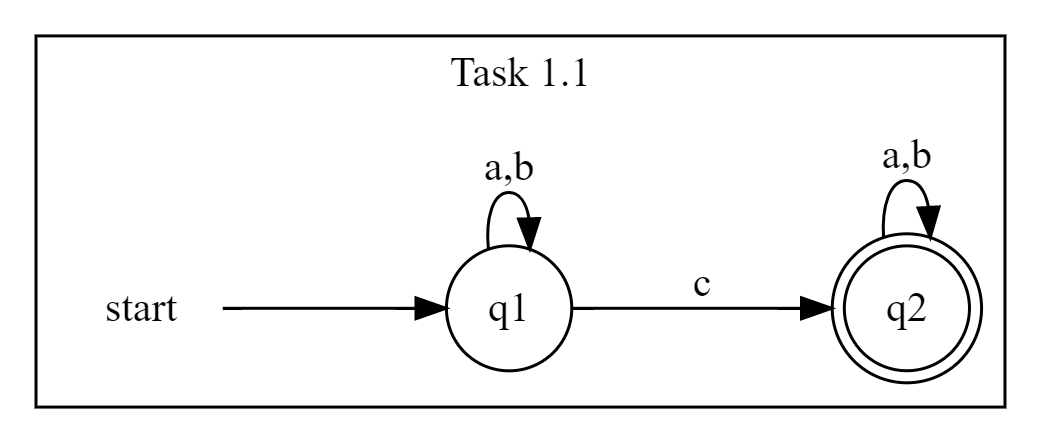
\includegraphics[scale=0.3]{1_1.png}

% 1.2
\subsection{L = \{ w \in ~  $\{a, b\}^*$ \mid  ~ $|w|_{a}$ \leq 2, $|w|_{b}$ \geq 2  \}}
\newline$L1 = \{ w \in \{ a, b\}^* | \quad |w|_a \leq 2\}$ \\
\newline\includegraphics[scale=0.3]{1_2_1.png}
\newline$L2 = \{ w \in \{ a, b\}^* | \quad |w|_b \geq 2 \}$\\
\newline\includegraphics[scale=0.3]{1_2_2.png}

\noindent\newline Переходы
\newline 
$\delta(q1p1, a) = q2p1$ \quad $\delta(q1p1, b) = q1p2$ \\
$\delta(q1p2, a) = q2p2$ \quad  $\delta(q1p0, b) = q1p3$ \\
$\delta(q1p3, a) = q2p3$ \quad  $\delta(q1p3, b) = q1p3$ \\
$\delta(q2p1, a) = q3p1$ \quad  $\delta(q2p1, b) = q2p2$ \\
$\delta(q2p2, a) = q3p2$ \quad  $\delta(q2p2, b) = q2p3$ \\
$\delta(q2p3, a) = q3p3$ \quad  $\delta(q2p3, b) = q2p3$ \\
$\delta(q3p1, a) = - $ \quad  $\delta(q3p1, b) = q3p2$ \\
$\delta(q3p2, a) = -$ \quad  $\delta(q3p2, b) = q3p3$ \\
$\delta(q3p3, a) = -$ \quad  $\delta(q3p3, b) = q3p3$ \\
\newline\includegraphics[scale=0.3]{1_2_3.png}


% 1.3
\subsection{L = \{ w \in ~  $\{a, b\}^*$ \mid ~ $|w|_{a}$ \neq $|w|_{b}$ \}^*}
Нельзя построить ДКА, так как требуется запоминать количество символов.

% 1.4
\subsection{L = \{ w \in ~  $\{a, b\}^*$ \mid  ww = www\}^*}
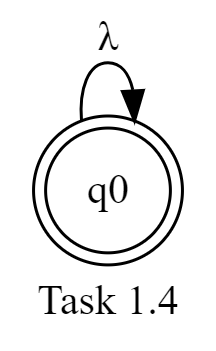
\includegraphics[scale=0.3]{1_4.png}

%---------------------------------------------------------
\section{Задание № 2. Построить конечный автомат, используя прямое произведение}
Ответом на данное задание является конечный автомат, распознающий описанный язык. Требуется, чтобы он был построен при помощи прямого произведения ДКА и его свойств.

% 2.1
\subsection{$L_{1}$ = \{ w \in ~  $\{a, b\}^*$ :  ~ $|w|_{a}$ \leq 2 ~ \wedge ~  $|w|_{b}$ \geq 2\}}
$A_{1}$=\{ w \in ~  $\{a, b\}^*$ :  ~ $|w|_{a}$ \geq 2 \}
\newline\includegraphics[scale=0.3]{2_1_1.png}

\newline$A_{2}$=\{ w \in ~  $\{a, b\}^*$ :  ~ $|w|_{b}$ \geq 2 \}
\newline\includegraphics[scale=0.3]{2_1_2.png}
\newline$L_{1}$ = $A_{1}$	\times $A_{2}$ 
\sum = \{a, b\}
\\Q = \{q1q4, q1q5, q1q6, q2q4, q2q5, q2q6, q3q4, q3q5, q3q6\}
\\S = \{q1q4\}
\\T = \{q3q6\}

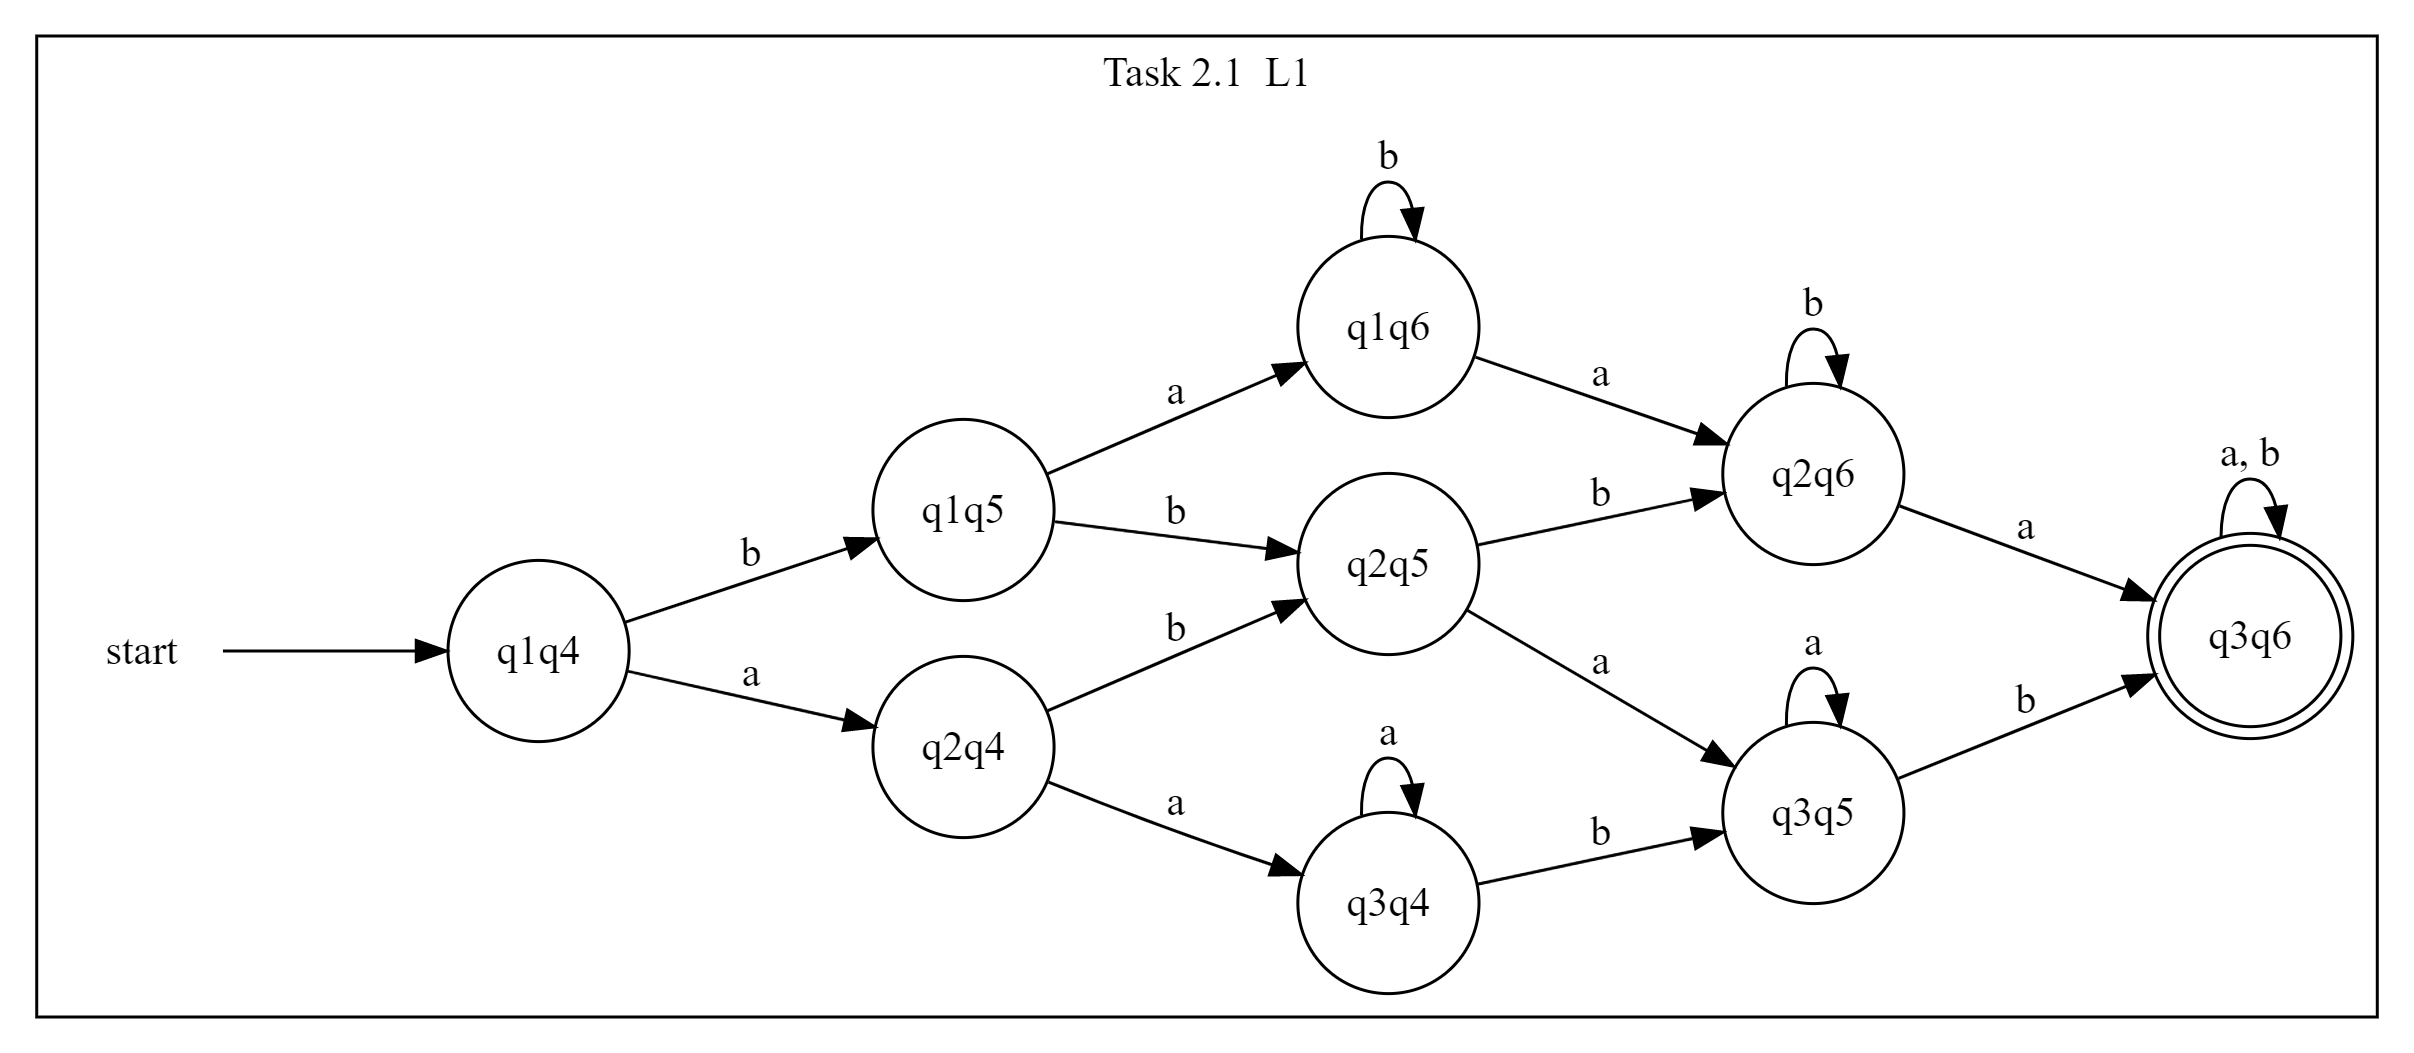
\includegraphics[scale=0.18]{2_1_3.png}

%2.2

\subsection{$L_2 = \{ w \in \{a,b\}^*$ | $  {|w|} \ge 3 \wedge {|w|} $ нечётное $ \} $}\\
Пусть:
$L_1_1$ = \{$ w \in \{a,b\}^*   $|$  {|w|} \ge 3 $ \} \\
\newline\includegraphics[scale=0.3]{2_2_1.png}
\newlineПусть:
$L_1_2$ = \{$ w \in \{a,b\}^*   $|$  {|w|} $ нечётное $ $ \} \\
\newline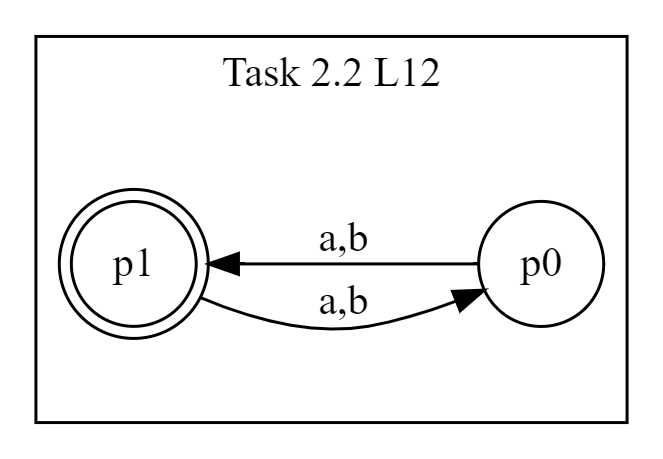
\includegraphics[scale=0.3]{2_2_2.png}

\noindent\newlineПрямое произведение $L_1_1$ \cap $L_1_2$.
\\где  $A_1_1 = (\sum_1 , Q_1, s_1, T_1, \delta_1) $ и  $A_1_2 = (\sum_2 , Q_2, s_2, T_2, \delta_2)$:\\
$\sum = \sum_1 \bigcup \sum_2 = \{a, b\}$\\
$Q = Q_1 \times Q_2$ $= \{q0p0, q0p1, q1p0, q1p1, q2p0, q2p1, q3p0, q3p1 \}$\\
$s = <s_1, s_2> = q0p0$\\
$T = T_1 \times T_2 = q3p1$\\
$ \delta(<q1, q2>, c) = <\delta_1(q_1, c), \delta_2(q_2, c)>$
\newline Переходы
\newline 
\noindent$\delta(q0p0, a) = q1p1$ \quad  $\delta(q0p0, b) = q1p1$ \\
\noindent$\delta(q0p1, a) = q1p0$ \quad $\delta(q0p1, b) = q1p0$ \\
\noindent$\delta(q1p0, a) = q2p1$ \quad  $\delta(q1p0, b) = q2p1$ \\
\noindent$\delta(q1p1, a) = q2p0$ \quad  $\delta(q1p1, b) = q2p0$ \\
\noindent$\delta(q2p0, a) = q3p1$ \quad  $\delta(q2p0, b) = q3p1$ \\
\noindent$\delta(q2p1, a) = q3p0$ \quad  $\delta(q2p1, b) = q3p0$ \\
\noindent$\delta(q3p0, a) = q3p1$ \quad  $\delta(q3p0, b) = q3p1$ \\
\noindent$\delta(q3p1, a) = q3p0$ \quad  $\delta(q3p1, b) = q3p0$ \\
\newline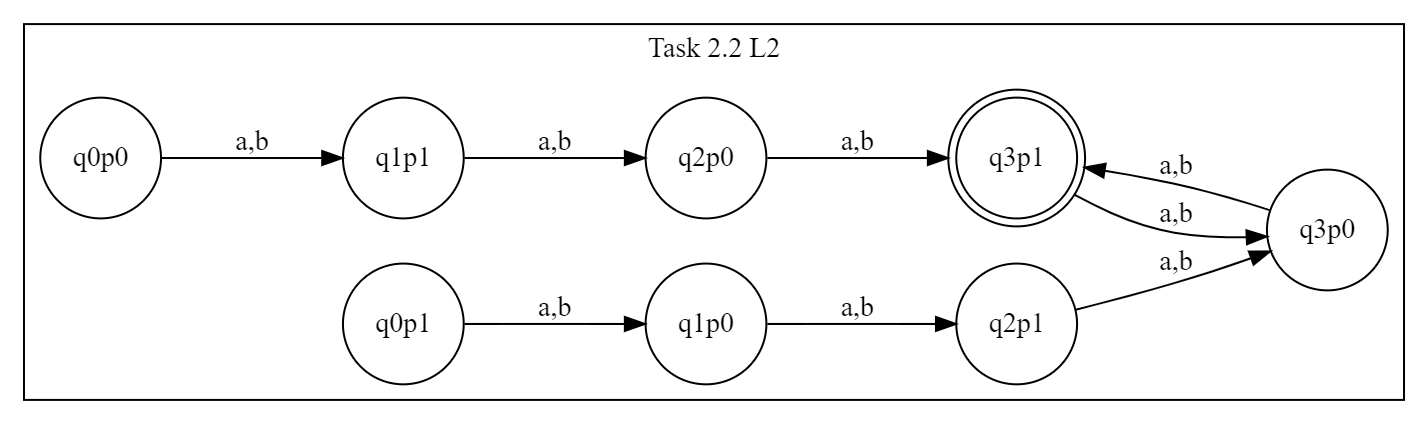
\includegraphics[scale=0.4]{2_2_3.png}

%2.3
\subsection{$L_3$ = \{ $w$ \in \{$a,b$\}$*$ $|$  $ {|w|_a}$ чётно  $\wedge$ ${|w|_b}$ кратно трём \} }\\

Пусть: 
$L_1_1$ = \{$ w \in \{a,b\}*   $|$  {|w|_a} $чётно$ $ \} \\
\newline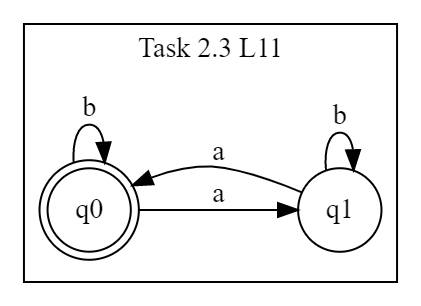
\includegraphics[scale=0.4]{2_3_1.png}
\\Пусть:
$L_1_2$ = \{$ w \in \{a,b\}*   $|$  {|w|_b} $ кратно трём $ $ \} \\
\newline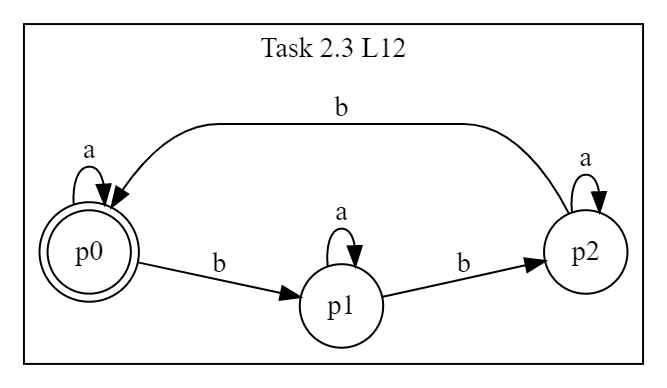
\includegraphics[scale=0.4]{2_3_2.png}
\\Прямое произведение  автоматов $L_3$ = $L_1_1$ \cap $L_1_2$.
\newline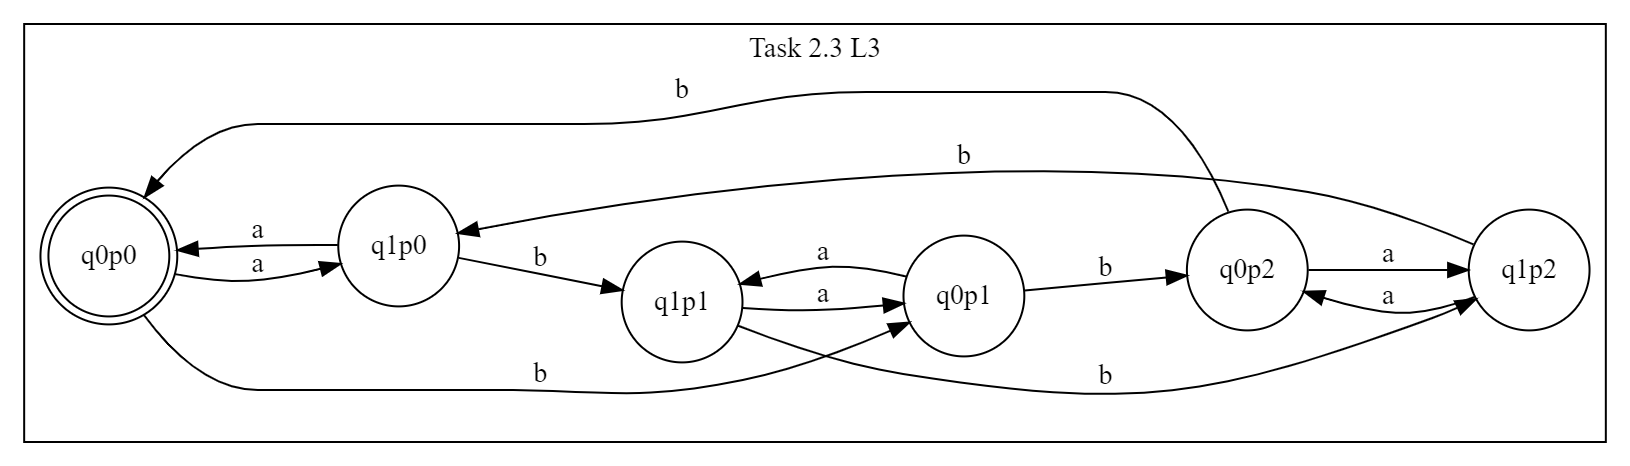
\includegraphics[scale=0.25]{2_3_3.png}

%2.4
\subsection {$L_4$ = $\overline{L_3}$}\\
$\sum = \sum_1 \bigcup \sum_2 = \{a, b\}$\\
$Q = Q_1 \times Q_2$ $= \{q0p0, q0p1, q0p2, q1p0, q1p1, q1p2 \}$\\
$s = <s_1, s_2> = q0p0$\\
$T = T_1 \times T_2 = q0p1, q0p2, q1p0, q1p1, q1p2 $\\
$ \delta(<q1, q2>, c) = <\delta_1(q_1, c), \delta_2(q_2, c)>$\\ 
\newline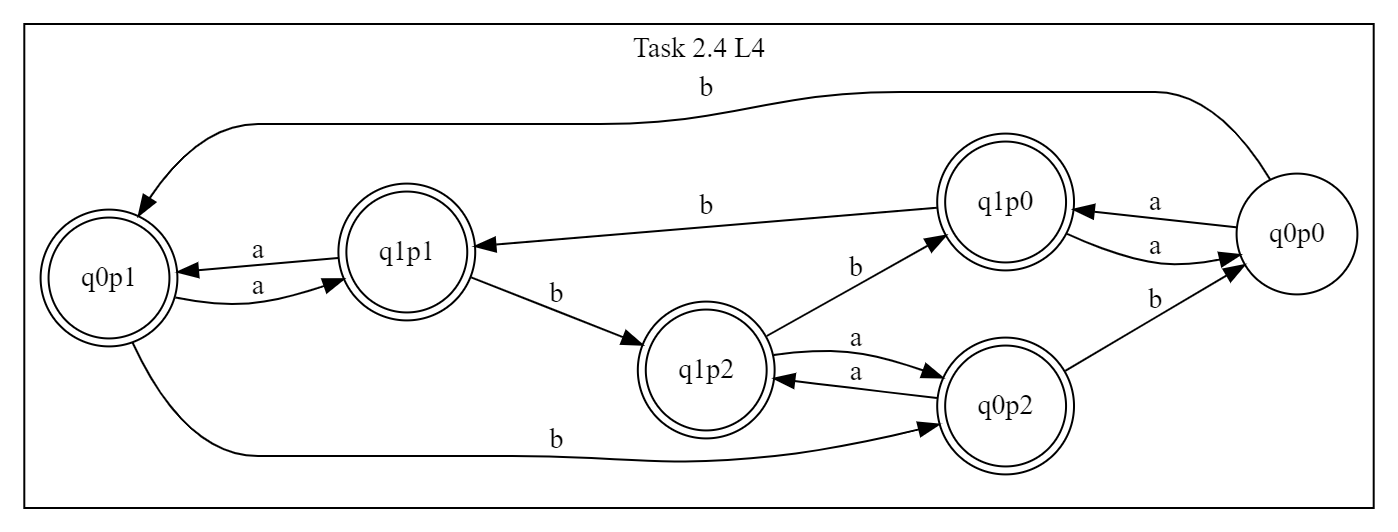
\includegraphics[scale=0.25]{2_4.png}


%2.5
\subsection{$L_5 = L_2 \setminus L_3 $}\\
$L_5 = L_2 \setminus L_3 $ $=$ $L_2 \cap \overline{L_3} = L_2 \times  \overline{L_3}$  $=$ $L_2$ \times $L_4$\\
Переобозначим вершины в автоматах для удобства
\\$L_2$:\\
\newline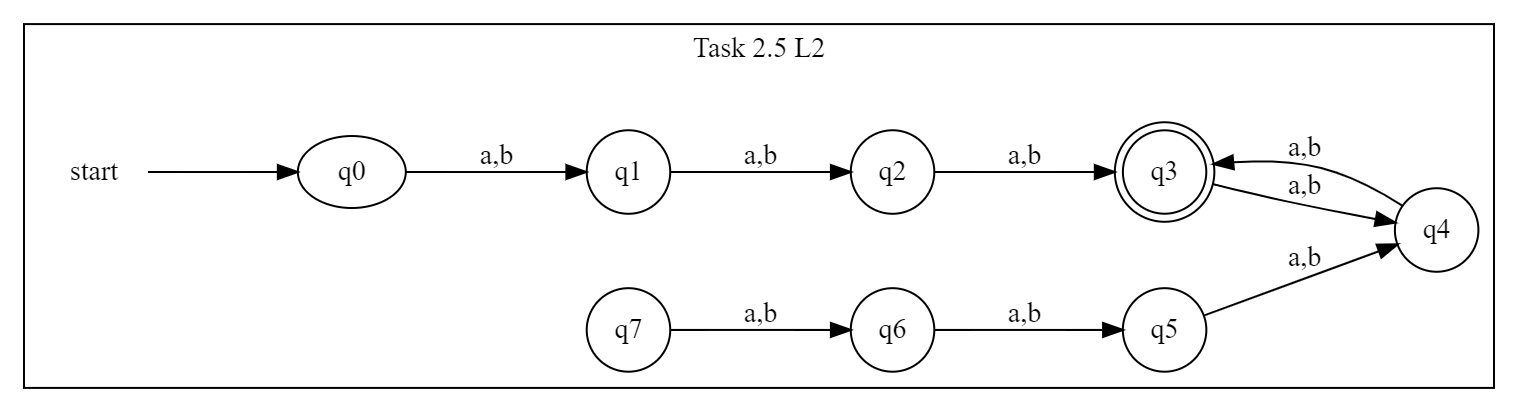
\includegraphics[scale=0.25]{2_5_1.png}
\\$L_4$:\\
\newline\includegraphics[scale=0.25]{2_5_2.png}

$\sum = \sum_1 \bigcup \sum_2 = \{a, b\}$\\
$Q = Q_1 \times Q_2$ $= \\
\{q0p0, \quad q0p1,\quad  q0p2,\quad q0p3,\quad q0p4, \quad q1p5,\\
q1p0, \quad q1p1, \quad  q1p2,\quad  q1p3, \quad q1p4, \quad q1p5,\\
q2p0,\quad q2p1,\quad q2p2, \quad q2p3,\quad q2p4,\quad q2p5,\\
q3p0, \quad q3p1, \quad q3p2,\quad  q3p3,\quad q3p4, \quad q3p5,\\
q4p0, \quad q4p1, \quad q4p2,\quad  q4p3,\quad q4p4,\quad q4p5,\\
q5p0,\quad q5p1,\quad q5p2,\quad q5p3,\quad q5p4,\quad q5p5,\\
q0p0,\quad q6p1,\quad q6p2,\quad q6p3,\quad q6p4,\quad q6p5,\\
q7p0,\quad q7p1,\quad q7p2,\quad q7p3,\quad q7p4,\quad q7p5\}
$\\
$s = <s_1, s_2> = q0p0$\\
$T = T_1 \times T_2 = q3p5, q3p2, q3p3, q3p4, q3p1 $\\
$ \delta(<q1, q2>, c) = <\delta_1(q_1, c), \delta_2(q_2, c)>$\\ 
\\Переходы $\delta$ \\ \\
\noindent$\delta(q0p0, a) = q1p1$ \  $\delta(q0p0, b) = q1p5$ \\
$\delta(q0p1, a) = q1p0$ \  $\delta(q0p1, b) = q1p4$ \\
$\delta(q0p2, a) = q1p3$ \  $\delta(q0p2, b) = q1p0$ \\
$\delta(q0p3, a) = q1p2$ \  $\delta(q0p3, b) = q1p1$ \\
$\delta(q0p4, a) = q1p5$ \  $\delta(q0p4, b) = q1p3$ \\
$\delta(q0p5, a) = q1p4$ \  $\delta(q0p5, b) = q1p2$ \\

\noindent$\delta(q1p0, a) = q2p1$ \  $\delta(q1p0, b) = q2p5$ \\
$\delta(q1p1, a) = q2p0$ \  $\delta(q1p1, b) = q2p4$ \\
$\delta(q1p2, a) = q2p3$ \  $\delta(q1p2, b) = q2p0$ \\
$\delta(q1p3, a) = q2p2$ \  $\delta(q1p3, b) = q2p1$ \\
$\delta(q1p4, a) = q2p5$ \  $\delta(q1p4, b) = q2p3$ \\
$\delta(q1p5, a) = q2p4$ \  $\delta(q1p5, b) = q2p2$ \\

\noindent$\delta(q2p0, a) = q3p1$ \  $\delta(q2p0, b) = q3p5$ \\
$\delta(q2p1, a) = q3p0$ \  $\delta(q2p1, b) = q3p4$ \\
$\delta(q2p2, a) = q3p3$ \  $\delta(q2p2, b) = q3p0$ \\
$\delta(q2p3, a) = q3p2$ \  $\delta(q2p3, b) = q3p1$ \\
$\delta(q2p4, a) = q3p5$ \  $\delta(q2p4, b) = q3p3$ \\
$\delta(q2p5, a) = q3p4$ \  $\delta(q2p5, b) = q3p2$ \\

\noindent$\delta(q3p0, a) = q4p1$ \  $\delta(q3p0, b) = q4p5$ \\
$\delta(q3p1, a) = q4p0$ \  $\delta(q3p1, b) = q4p4$ \\
$\delta(q3p2, a) = q4p3$ \  $\delta(q3p2, b) = q4p0$ \\
$\delta(q3p3, a) = q4p2$ \  $\delta(q3p3, b) = q4p1$ \\
$\delta(q3p4, a) = q4p5$ \  $\delta(q3p4, b) = q4p3$ \\
$\delta(q3p5, a) = q4p4$ \  $\delta(q3p5, b) = q4p2$ \\

\noindent$\delta(q4p0, a) = q3p1$ \  $\delta(q4p0, b) = q3p5$ \\
$\delta(q4p1, a) = q3p0$ \  $\delta(q4p1, b) = q3p4$ \\
$\delta(q4p2, a) = q3p3$ \  $\delta(q4p2, b) = q3p0$ \\
$\delta(q4p3, a) = q3p2$ \  $\delta(q4p3, b) = q3p1$ \\
$\delta(q4p4, a) = q3p5$ \  $\delta(q4p4, b) = q3p3$ \\
$\delta(q4p5, a) = q3p4$ \  $\delta(q4p5, b) = q3p2$ \\

\noindent$\delta(q5p0, a) = q4p1$ \  $\delta(q5p0, b) = q4p5$ \\
$\delta(q5p1, a) = q4p0$ \  $\delta(q5p1, b) = q4p4$ \\
$\delta(q5p2, a) = q4p3$ \  $\delta(q5p2, b) = q4p0$ \\
$\delta(q5p3, a) = q4p2$ \  $\delta(q5p3, b) = q4p1$ \\
$\delta(q5p4, a) = q4p5$ \  $\delta(q5p4, b) = q4p3$ \\
$\delta(q5p5, a) = q4p4$ \  $\delta(q5p5, b) = q4p2$ \\

\noindent$\delta(q5p0, a) = q4p1$ \  $\delta(q5p0, b) = q4p5$ \\
$\delta(q5p1, a) = q4p0$ \  $\delta(q5p1, b) = q4p4$ \\
$\delta(q5p2, a) = q4p3$ \  $\delta(q5p2, b) = q4p0$ \\
$\delta(q5p3, a) = q4p2$ \  $\delta(q5p3, b) = q4p1$ \\
$\delta(q5p4, a) = q4p5$ \  $\delta(q5p4, b) = q4p3$ \\
$\delta(q5p5, a) = q4p4$ \  $\delta(q5p5, b) = q4p2$ \\

\noindent$\delta(q6p0, a) = q5p1$ \  $\delta(q6p0, b) = q5p5$ \\
$\delta(q6p1, a) = q5p0$ \  $\delta(q6p1, b) = q5p4$ \\
$\delta(q6p2, a) = q5p3$ \  $\delta(q6p2, b) = q5p0$ \\
$\delta(q6p3, a) = q5p2$ \  $\delta(q6p3, b) = q5p1$ \\
$\delta(q6p4, a) = q5p5$ \  $\delta(q6p4, b) = q5p3$ \\
$\delta(q6p5, a) = q5p4$ \  $\delta(q6p5, b) = q5p2$ \\

\noindent$\delta(q7p0, a) = q6p1$ \  $\delta(q7p0, b) = q6p5$ \\
$\delta(q7p1, a) = q6p0$ \  $\delta(q7p1, b) = q6p4$ \\
$\delta(q7p2, a) = q6p3$ \  $\delta(q7p2, b) = q6p0$ \\
$\delta(q7p3, a) = q6p2$ \  $\delta(q7p3, b) = q6p1$ \\
$\delta(q7p4, a) = q6p5$ \  $\delta(q7p4, b) = q6p3$ \\
$\delta(q7p5, a) = q6p4$ \  $\delta(q7p5, b) = q6p2$ \\

\newpage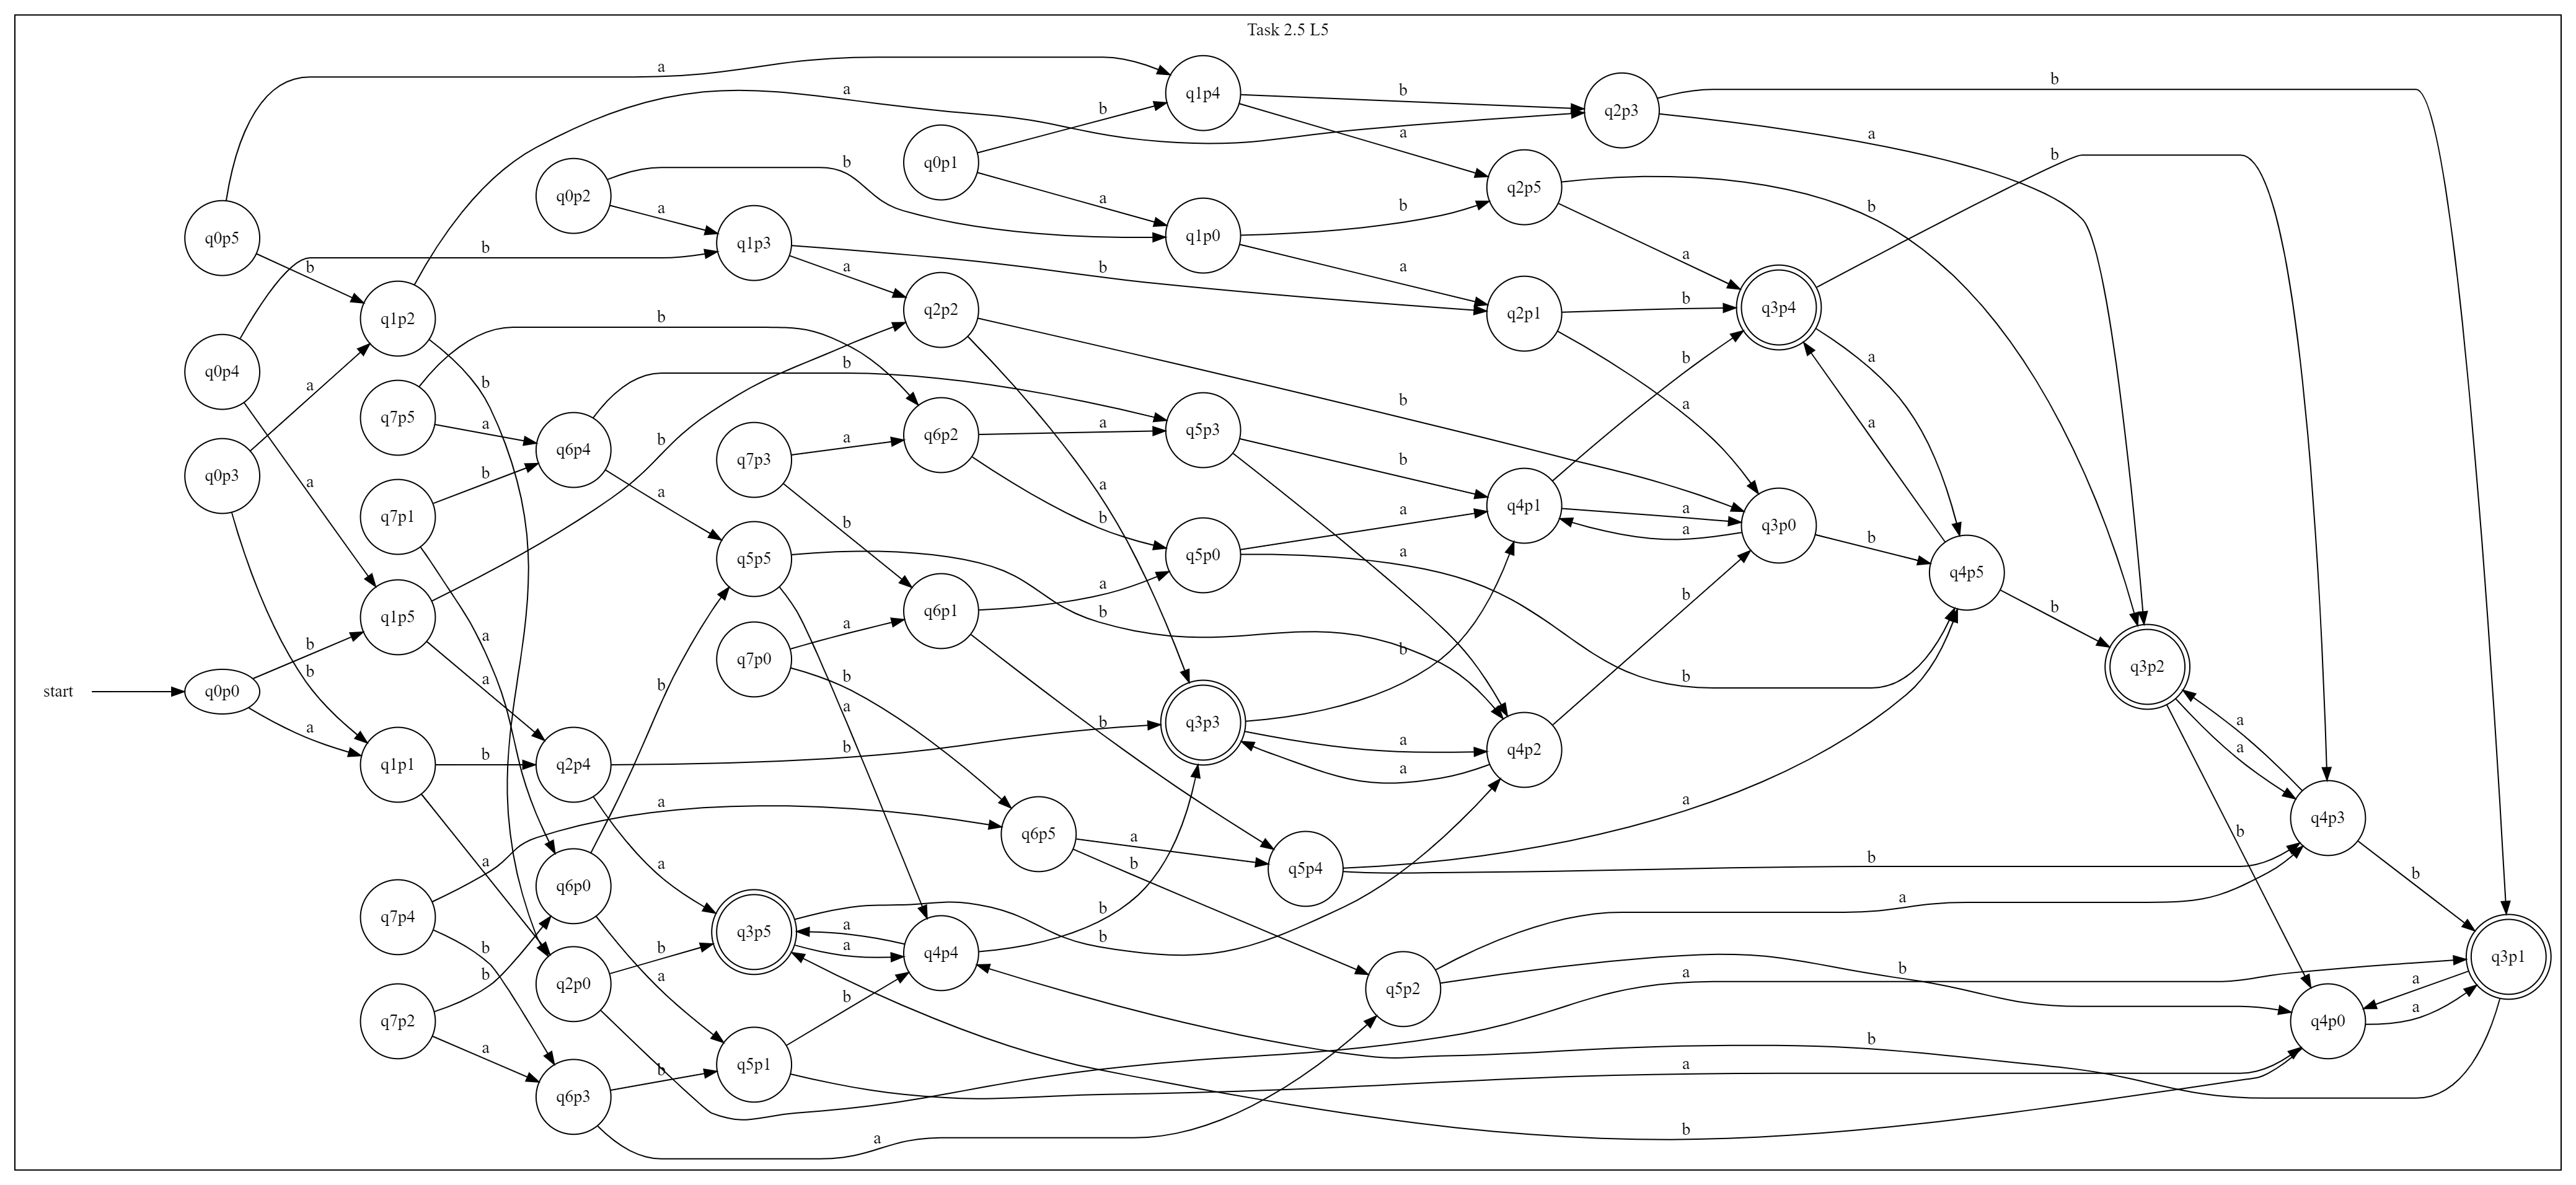
\includegraphics[scale=0.18]{2_5_3.png}
%\begin{landscape}
%поворот текста
%\end{landscape}

%---------------------------------------------------------
%3

%3.1
\newpage\section{Задание №3. Построить минимальный ДКА по регулярному выражению}
\subsection{$ (ab + aba)^*a $}\\ 
\newline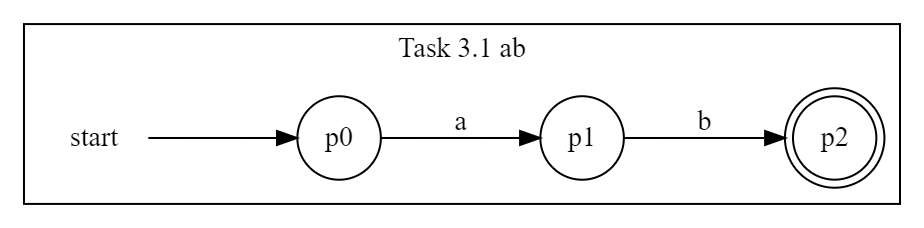
\includegraphics[scale=0.4]{3_1_1.png}
\newline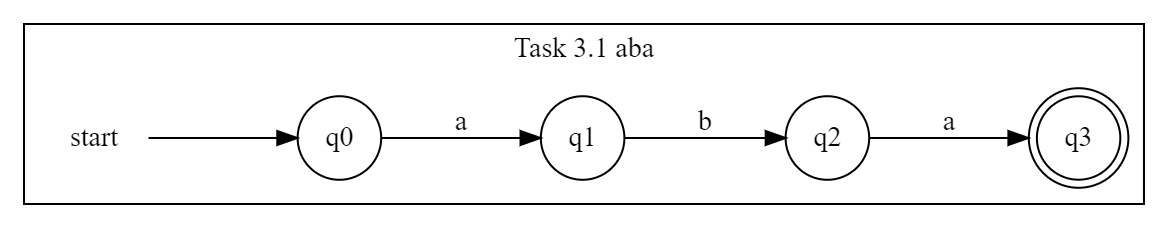
\includegraphics[scale=0.4]{3_1_2.png}
\newline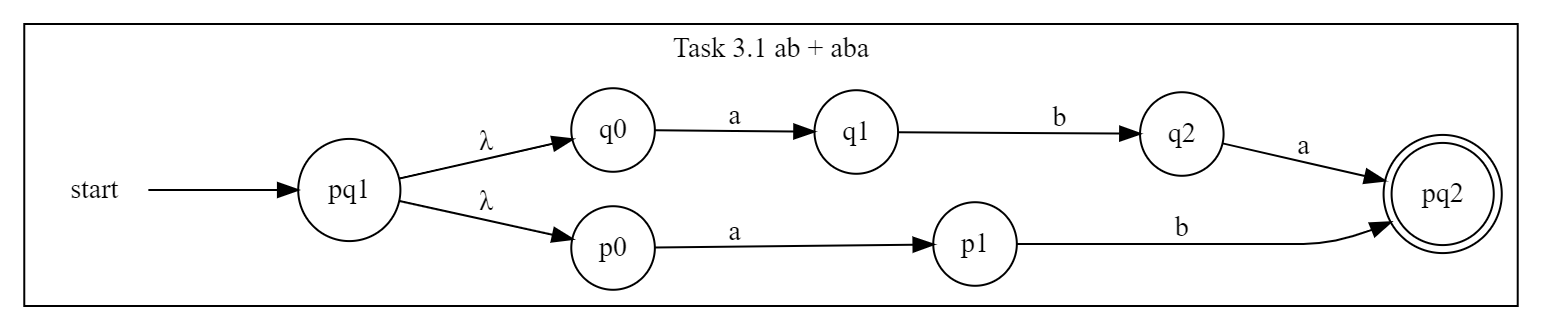
\includegraphics[scale=0.4]{3_1_3.png} 
\newline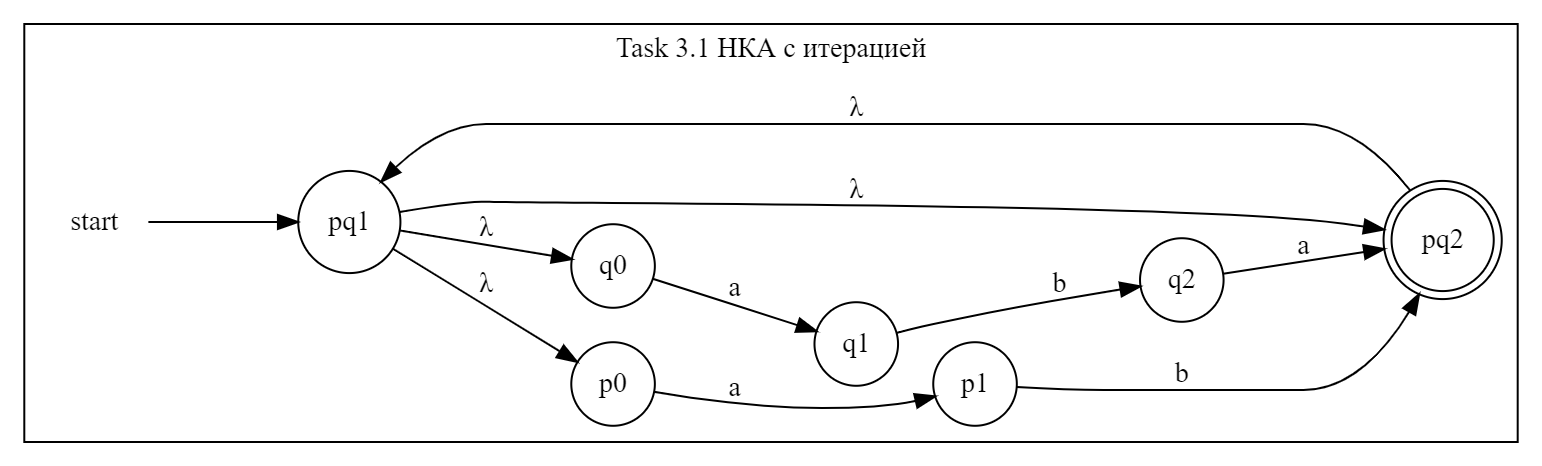
\includegraphics[scale=0.4]{3_1_4.png} 
\newline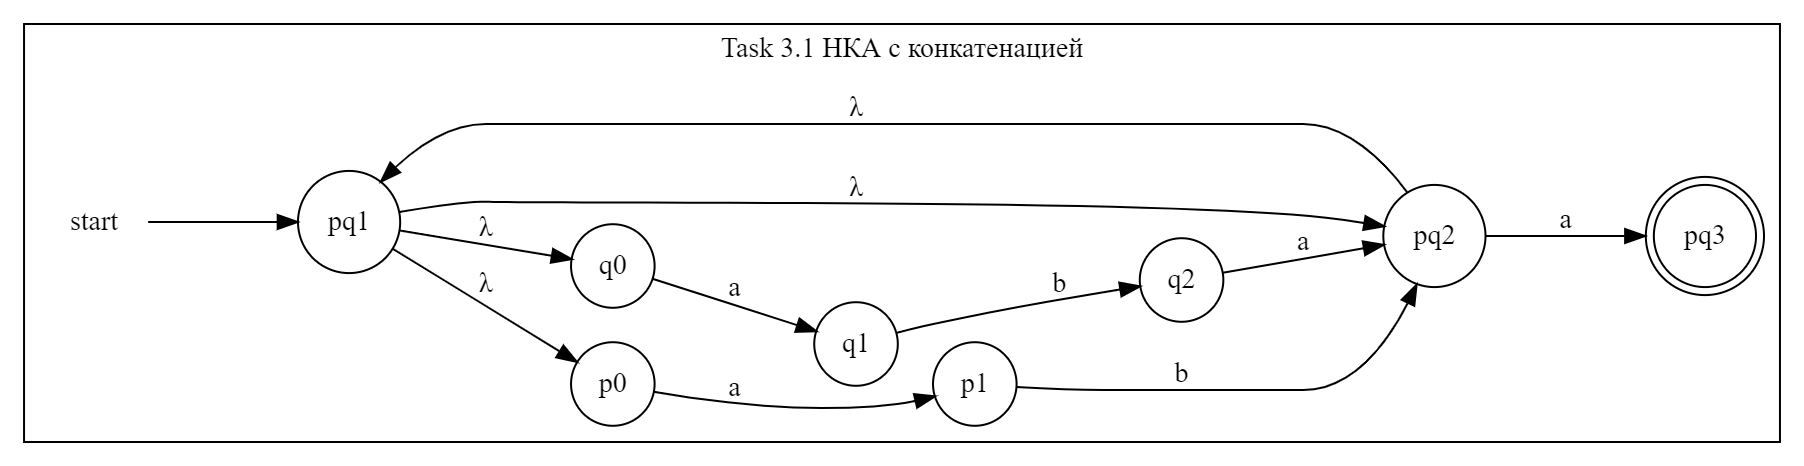
\includegraphics[scale=0.4]{3_1_5.png}
После удаления $\lambda$-переходов:
\newline\includegraphics[scale=0.4]{3_1_6.png}

%3.2
\subsection{$a(a(ab)^* b)^* (ab)^*$}
\newline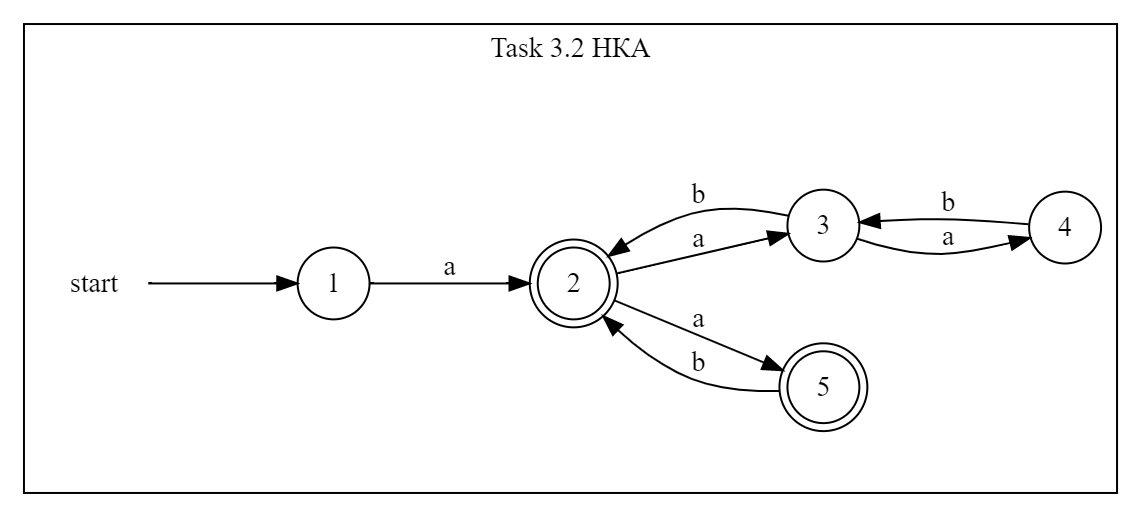
\includegraphics[scale=0.4]{3_2_1.png}
\newline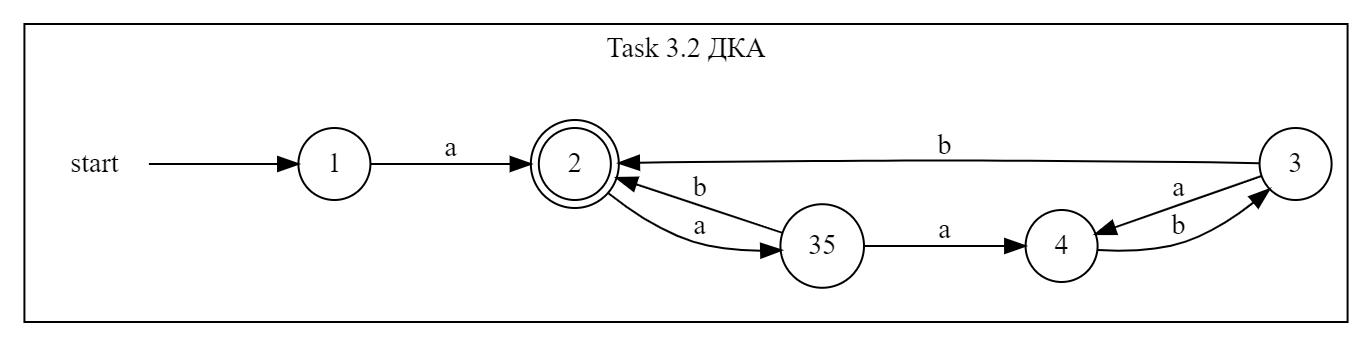
\includegraphics[scale=0.4]{3_2_2.png}
\newline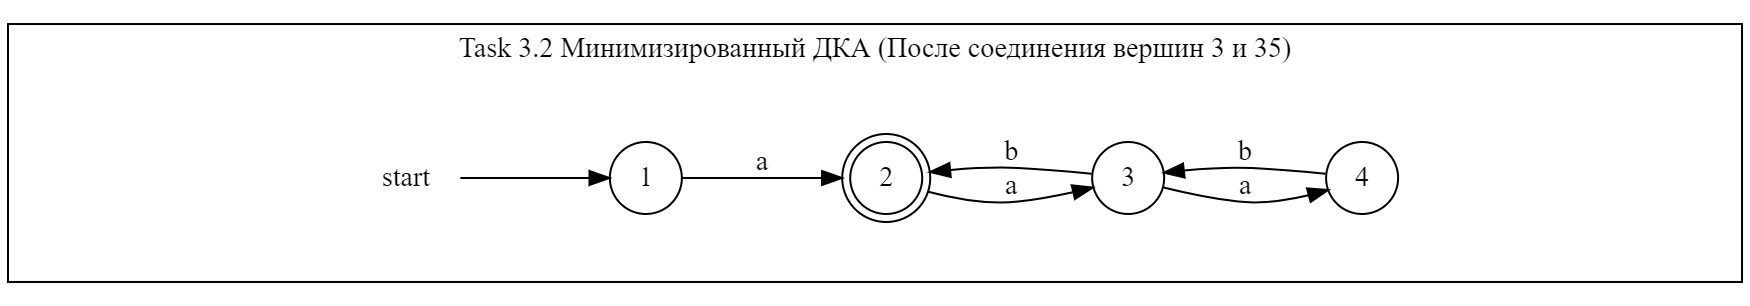
\includegraphics[scale=0.4]{3_2_3.png}
 
%3.3
\subsection{$ (a + (a + b)(a + b)b)^*$}\\ 
\newline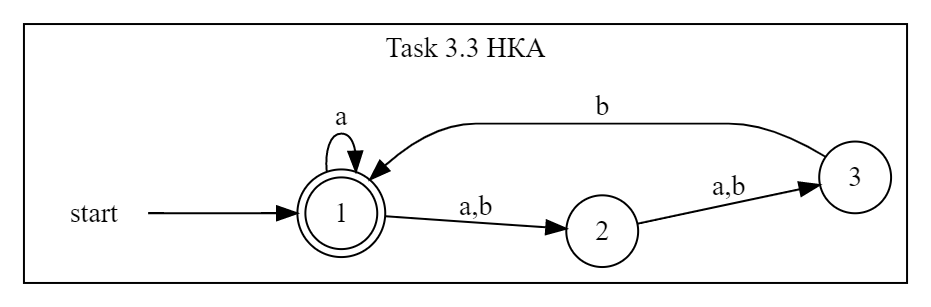
\includegraphics[scale=0.4]{3_3_1.png}

\noindentПереходы
\newline $\delta(1, a) = 12  \quad  ~~ \;$\delta(1, b) = 2$ \\
$\delta(12, a) = 123$        \quad  $\delta(12, b) = 23$ \\
$\delta(2, a) = 3$ \quad  ~ ~ $\delta(2, b) = 3$ \\
$\delta(123, a) = 123$  ~  $\delta(123, b) = 123$ \\
$\delta(23, a) = 3$ \quad ~ $\delta(23, b) = 13$ \\
$\delta(3, a) = -$ \quad  ~$\delta(3, b) = 1$ \\
$\delta(13, a) = 12$ \quad  ~$\delta(13, b) = 12$ \\
\newline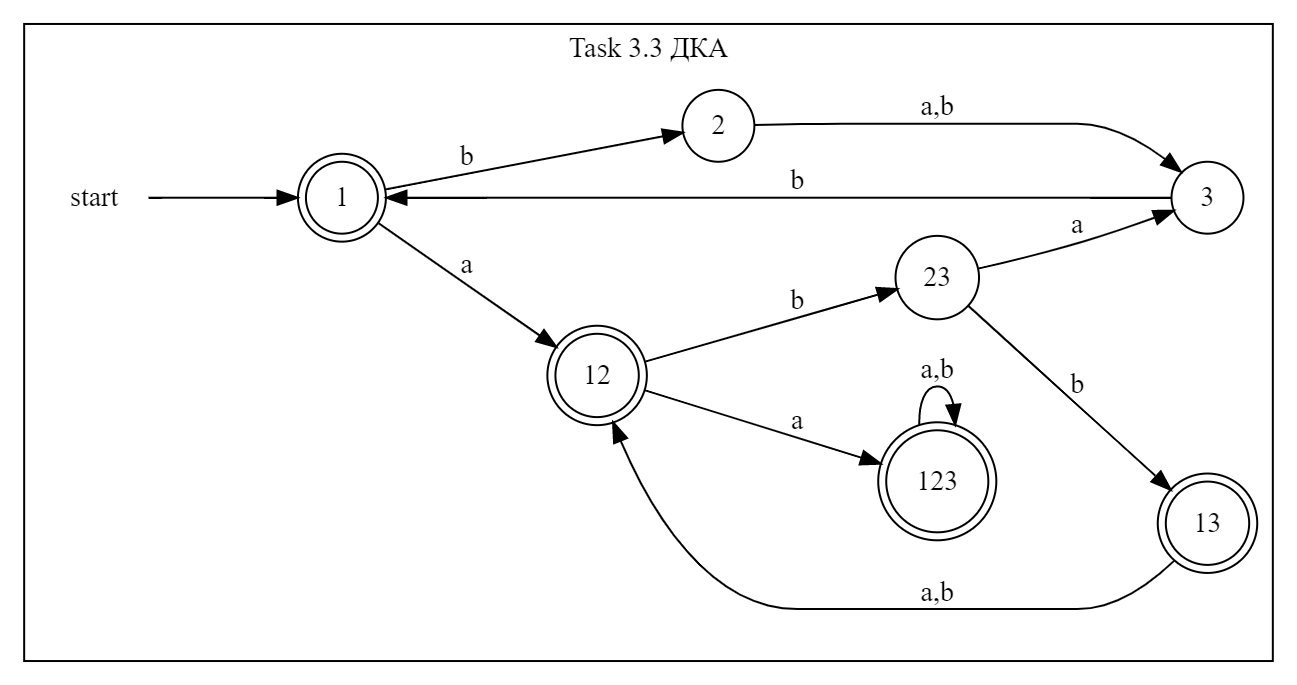
\includegraphics[scale=0.4]{3_3_2.png}

\noindent\\Классы эквивалентности:
\newline k0:\{1,12,123,13\} \{23,2,3\}
\newline k1:\{1,12\} \{123,13\} \{23\} \{3\} \{2\}
\newline k2:\{1\} \{12\} \{123\} \{13\} \{23\} \{3\} \{2\}

\noindent\\Таким образом, построенный автомат минимален.

%3.4
\subsection{$ (b+c)((ab)^*c + (ba)^*)^*$}\\ 
\newline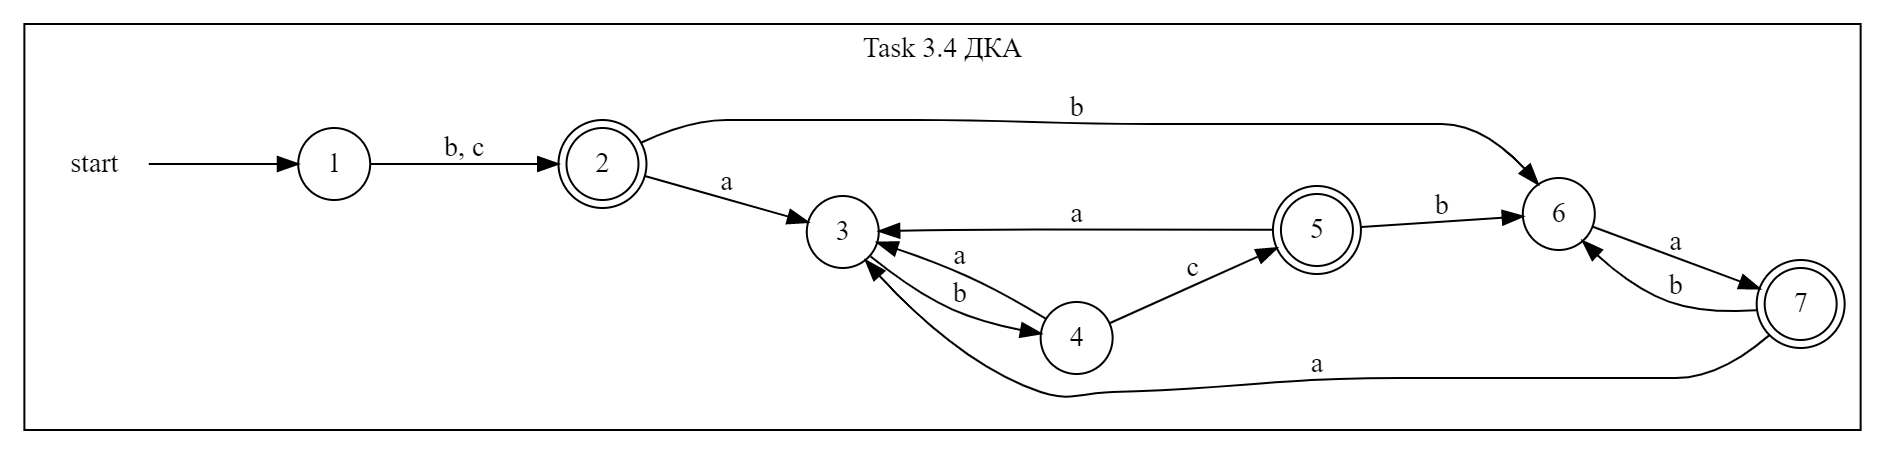
\includegraphics[scale=0.4]{3_4_1.png}
\newline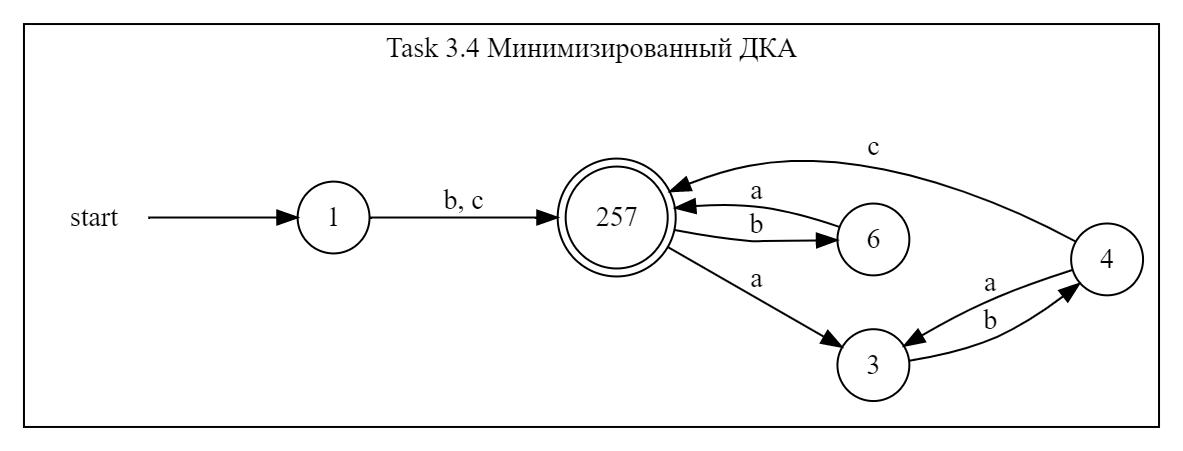
\includegraphics[scale=0.4]{3_4_2.png}  


%3.5
\subsection{$ (a+b)^+(aa + abab + bb + baba)(a+b)^+$}\\ 
\newline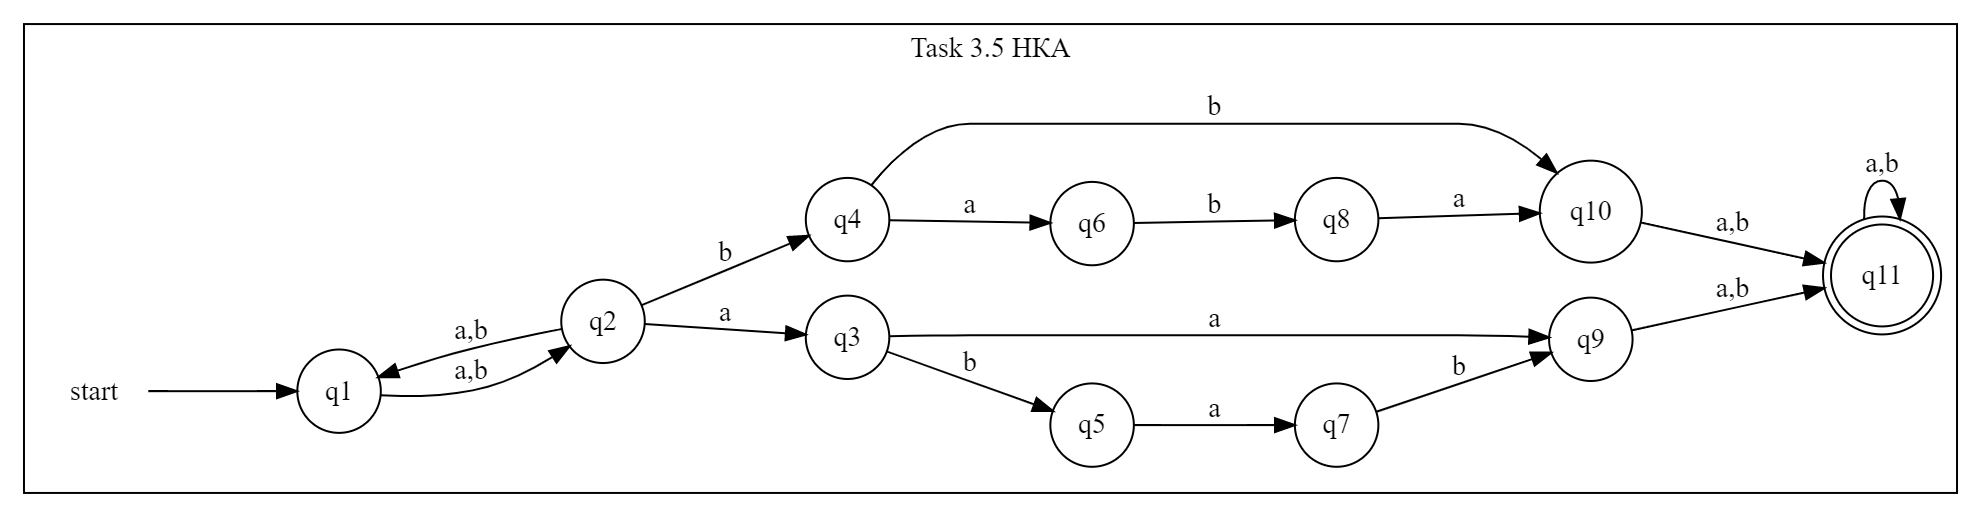
\includegraphics[scale=0.3]{3_5_1.png}      
\newline Эквивалентный ДКА:
\newline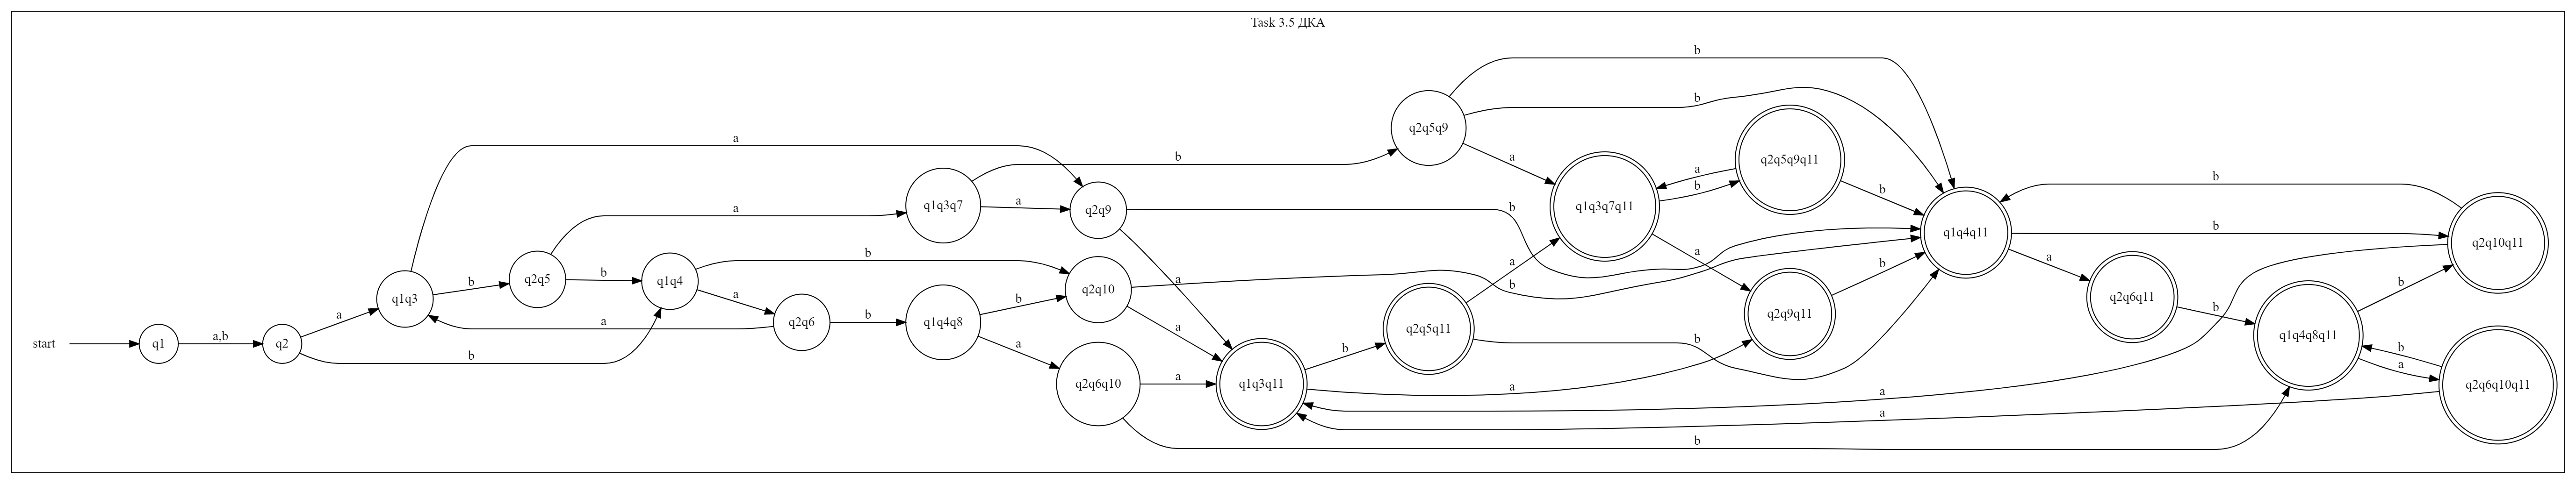
\includegraphics[scale=0.14]{3_5_2.png} 
\newline Минимизированный ДКА:
\newline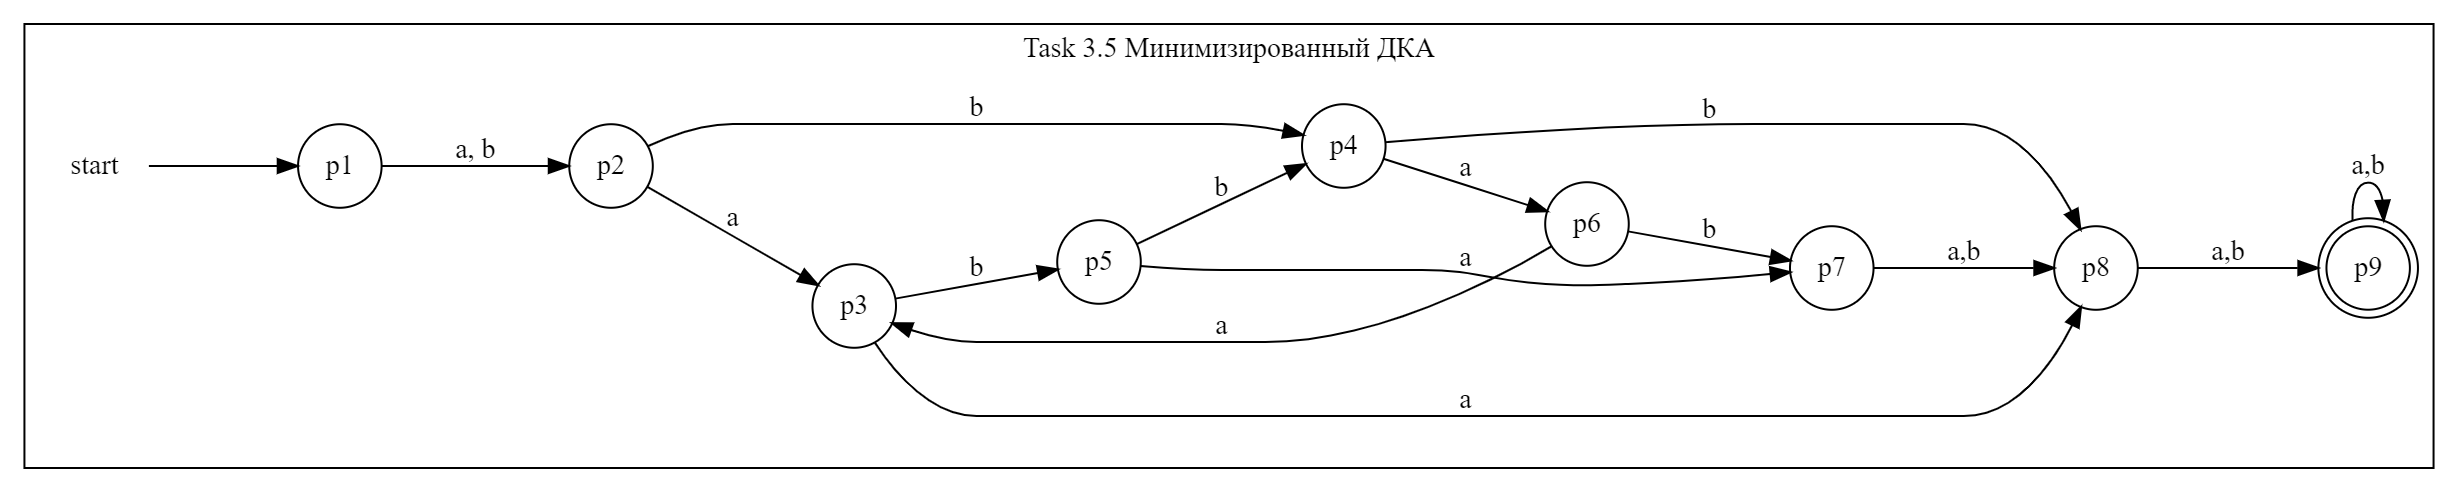
\includegraphics[scale=0.3]{3_5_3.png}   

%---------------------------------------------------------
% 4
\newpage\section{Задание №4. Определить является ли язык регулярным или нет.}
% 4.1
\subsection{$L = \{(aab)^n b(aba)^m  $ | $ $ n \ge 0, m \ge 0 \}}\\ 
Построим ДКА
\newline\includegraphics[scale=0.3]{4_1.png}  
\newlineТаким образом, язык является регулярным.
% 4.2
\subsection{$L = \{ uaav  | u \in \{a,b\}^* ,  v \in \{a, b\}^* |u|_b\ge|u|_a  \}$}\\
Доказывать будем методом от противного.
Предположим, что язык регулярен . Используем лемму о разрастании.
Рассмотрим некоторое слово
$w = b^naaa^n, |w| = 2n+2 \ge n.$\\
$w = xyz, |y| \ne 0, |xy| \le n:$\\
$x = b^i, y = b^j, z = b^{n-i-j}aaa^n$\\
$i + j \le n, j \ne 0 $\\
$w = xy^kz=b^ib^{lj}b^{n-i-j}aaa^n$\\
Пусть $l=0,$ тогда: $w = b^{n-j}aaa^n \notin L  ,j \ne 0$\\
Лемма не выполняется, следовательно, исходное предположение неверно, язык не является регулярным\\
%4.3
\subsection{$L = \{ a^mw  | w \in \{a,b\}^* , 1 \le |w|_b \le m   \} $}\\
\\ Используем лемму о разрастании\\
Предположим, что язык регулярен.
Рассмотрим некоторое слово
$w = a^nb^n, |w| = 2n \ge n.$\\
$w = xyz, |y| \ne 0, |xy| \le n:$\\
$x = a^i, y = a^j, z = a^{n-i-j}b^n$\\
$i + j \le n, j \ne 0 $\\
$w = xy^kz=a^ia^{lj}a^{n-i-j}b^n$\\
Пусть $l=0,$ тогда: $w = a^{n-j}b^n \notin L  ,j \ne 0$\\
Лемма не выполняется, следовательно, исходное предположение неверно, язык не является регулярным\\
%4.4
\subsection{$L = \{ a^kb^ma^n  | k = n \vee m > 0  \} $}\\
\\ Используем лемму о разрастании\\
Предположим, что язык регулярен. Рассмотрим некоторое слово
$w = a^nba^n, |w| = 2n+1 \ge n.$\\
$w = xyz, |y| \ne 0, |xy| \le n:$\\
$x = a^i, y = a^j, z = a^{n-i-j}ba^n$\\
$i + j \le n, j \ne 0 $\\
$w = xy^kz=a^ia^{lj}a^{n-i-j}ba^n$\\
Пусть $l=2,$ тогда: $w = a^{n+j}ba^n \notin L  ,j \ne 0$\\
Лемма не выполняется, следовательно, исходное предположение неверно, язык не является регулярным\\

%4.5
\subsection{$L = \{ ucv  | u \in \{a,b\}^*, v \in \{a,b\}^* , u \ne v^R\} $}\\
\\ Используем лемму о разрастании\\
Предположим, что язык регулярен.\\ Рассмотрим некоторое слово
\\$w =(ab)^nc(ab)^n = \alpha_1 \alpha_2 ... \alpha_n...\alpha_{2n}...\alpha_{4n}\alpha_{4n+1}, |w| = 4n+1 \ge n.$\\
$w = xyz, |y| \ne 0, |xy| \le n:$\\
$x = \alpha_1 \alpha_2...\alpha_i, y = \alpha_{i+1} \alpha_{i+2}...\alpha_{i+j}, z = \alpha_{i+j+1}\alpha_{i+j+2}...\alpha_{4n+1}c(ab)^n$\\
$i + j \le n, j \ne 0 $\\
$w = xy^lz=(\alpha_1 \alpha_2...\alpha_i)(\alpha_{i+1} \alpha_{i+2}...\alpha_{i+j})^l(\alpha_{i+j+1}\alpha_{i+j+2}...\alpha_{4n+1}c(ab)^n)$\\
\\
Пусть $l=2,$ тогда: $w = (\alpha_1 \alpha_2...\alpha_i)(\alpha_{i+1} \alpha_{i+2}...\alpha_{i+j})^2(\alpha_{i+j+1}\alpha_{i+j+2}...\alpha_{4n+1}c(ab)^n) \notin L  ,j \ne 0$\\
Лемма не выполняется, следовательно, исходное предположение неверно, язык не является регулярным\\


\end{document}
